% Native editable composition from verified, unchanged IDE images.
\par
\begin{figure}[htbp]
\centering
\sbox0{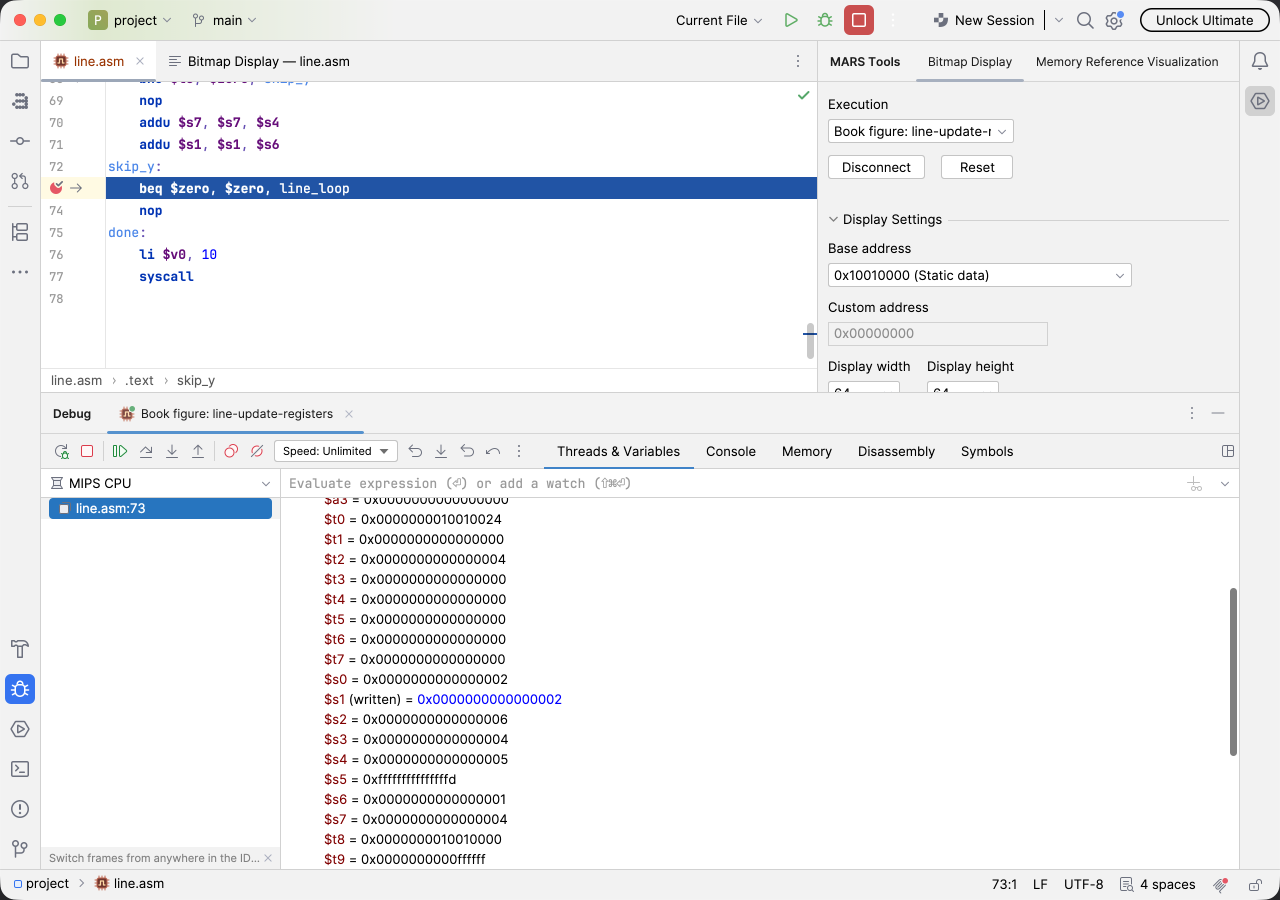
\includegraphics[artifact]{packages/007-bresenham-line/captures/f02-update/registers.png}}
\sbox2{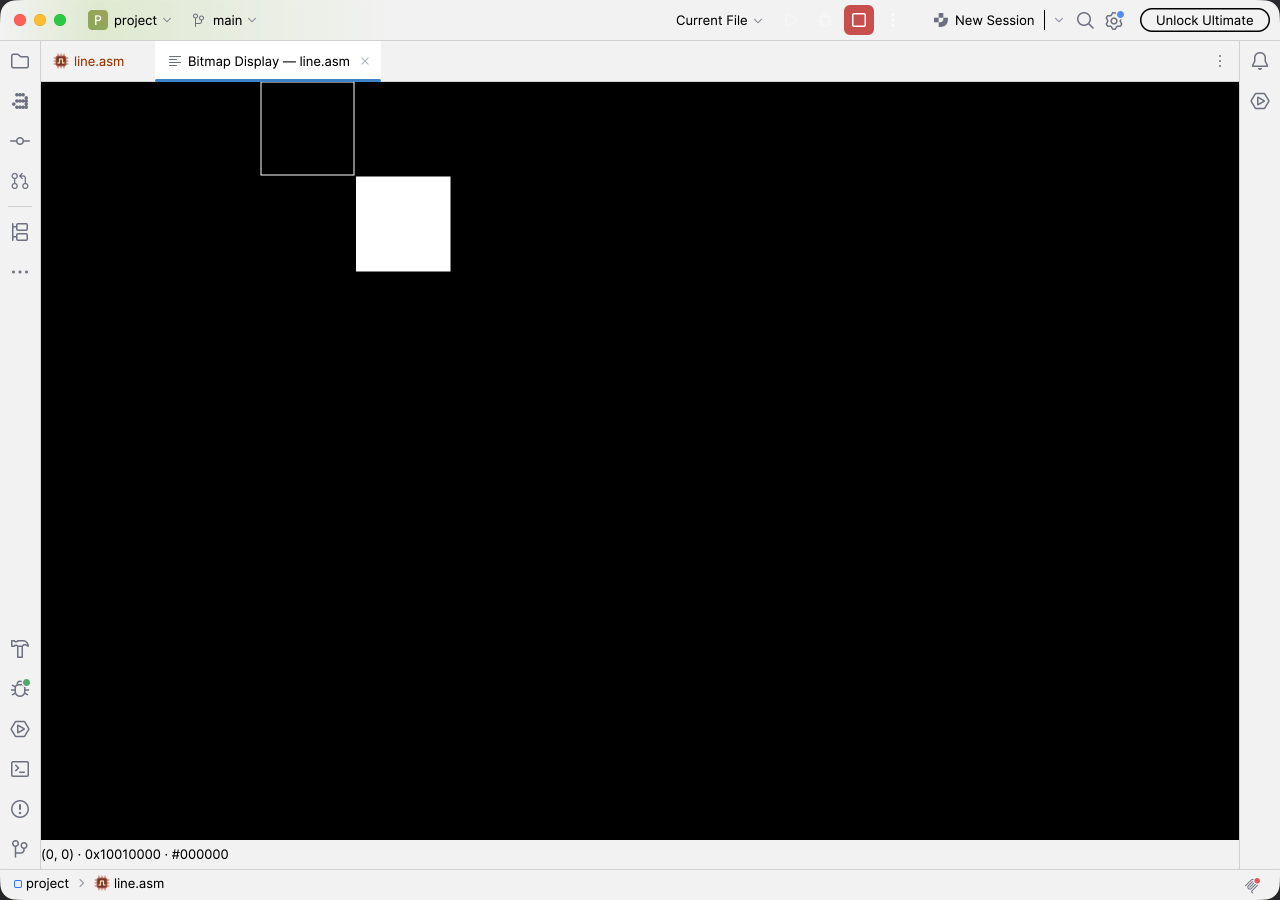
\includegraphics[artifact]{packages/007-bresenham-line/captures/f02-update/bitmap.png}}
\edef\MARSupdatesourceLeft{\the\dimexpr0.036718750\wd0\relax}
\edef\MARSupdatesourceBottom{\the\dimexpr0.774444444\ht0\relax}
\edef\MARSupdatesourceRight{\the\dimexpr0.611718750\wd0\relax}
\edef\MARSupdatesourceTop{\the\dimexpr0.147777778\ht0\relax}
\edef\MARSupdatestateLeft{\the\dimexpr0.246093750\wd0\relax}
\edef\MARSupdatestateBottom{\the\dimexpr0.075555556\ht0\relax}
\edef\MARSupdatestateRight{\the\dimexpr0.554687500\wd0\relax}
\edef\MARSupdatestateTop{\the\dimexpr0.740000000\ht0\relax}
\edef\MARSupdateplotLeft{\the\dimexpr0.203906250\wd2\relax}
\edef\MARSupdateplotBottom{\the\dimexpr0.066666667\ht2\relax}
\edef\MARSupdateplotRight{\the\dimexpr0.203906250\wd2\relax}
\edef\MARSupdateplotTop{\the\dimexpr0.091111111\ht2\relax}
\edef\MARSupdatesavedLeft{\the\dimexpr0.246093750\wd0\relax}
\edef\MARSupdatesavedBottom{\the\dimexpr0.364444444\ht0\relax}
\edef\MARSupdatesavedRight{\the\dimexpr0.598437500\wd0\relax}
\edef\MARSupdatesavedTop{\the\dimexpr0.606666667\ht0\relax}
\begin{tikzpicture}[alt={Four annotated details at skip y after the first update. The next branch returns to the line loop. Working x and y are two and two, running error is four, and saved doubled error t2 is four from the earlier error two. The original bitmap still has only cell one one white.}]
\node[anchor=north west,inner sep=0,font=\small\bfseries] (source-title) at (6mm,0) {The next branch returns to the drawing loop};
\node[anchor=north west,inner sep=0] (source) at ([yshift=-1mm]source-title.south west) {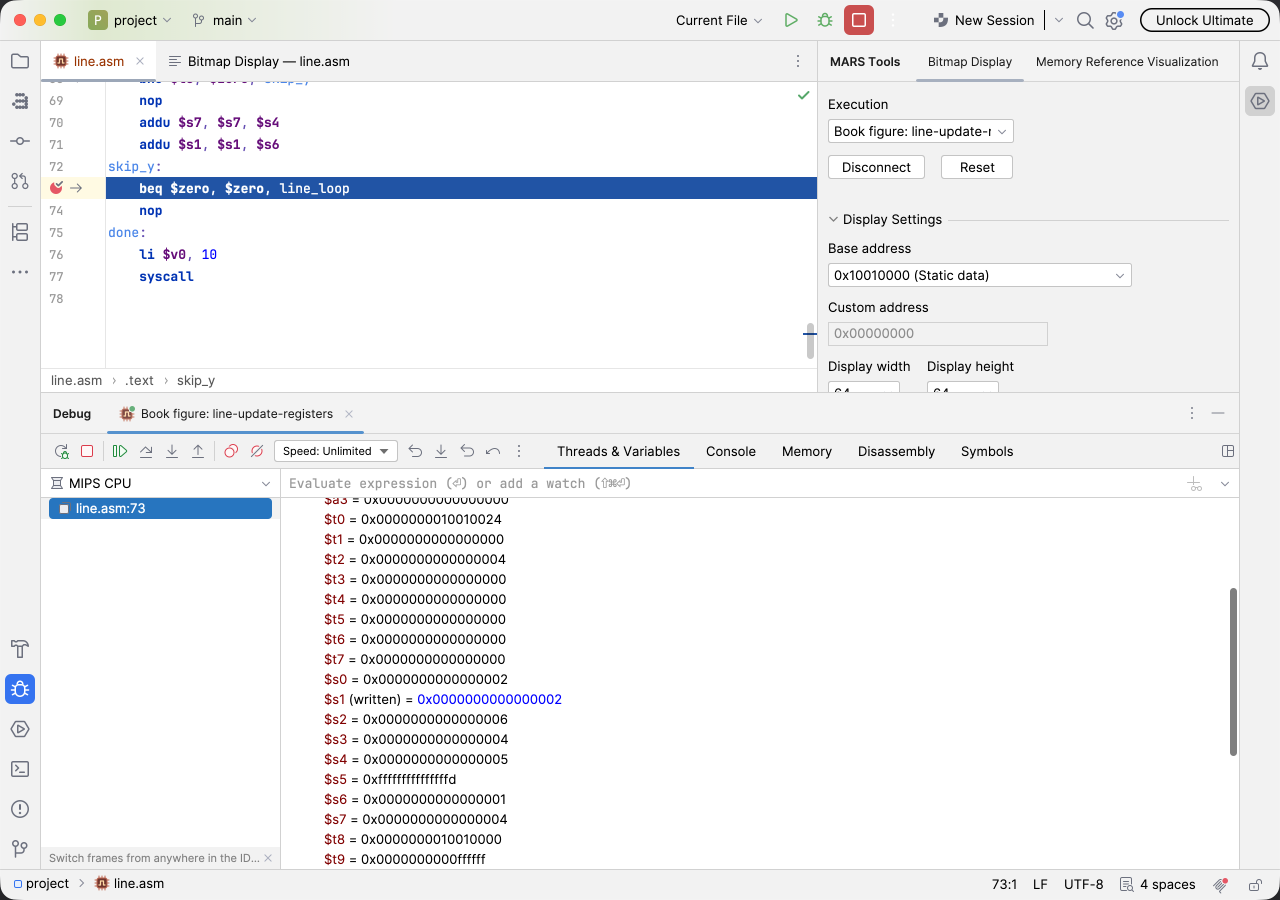
\includegraphics[width=0.7\linewidth,artifact,trim={\MARSupdatesourceLeft{} \MARSupdatesourceBottom{} \MARSupdatesourceRight{} \MARSupdatesourceTop{}},clip]{packages/007-bresenham-line/captures/f02-update/registers.png}};
\begin{scope}[shift={(source.south west)},x={($(source.south east)-(source.south west)$)},y={($(source.north west)-(source.south west)$)}]
\draw[black,line width=0.7pt] (0.135555556,0.057142857) rectangle (0.671111111,0.371428571);
\node[draw=black,fill=white,circle,inner sep=1.5pt,font=\footnotesize] at ($(0.135555556,0.371428571)+(-3mm,0)$) {1};
\end{scope}
\node[anchor=north west,inner sep=0,font=\small\bfseries] (state-title) at ([yshift=-2mm]source.south west) {A prepared coordinate is not a completed store};
\node[anchor=north west,inner sep=0] (state) at ([yshift=-1mm]state-title.south west) {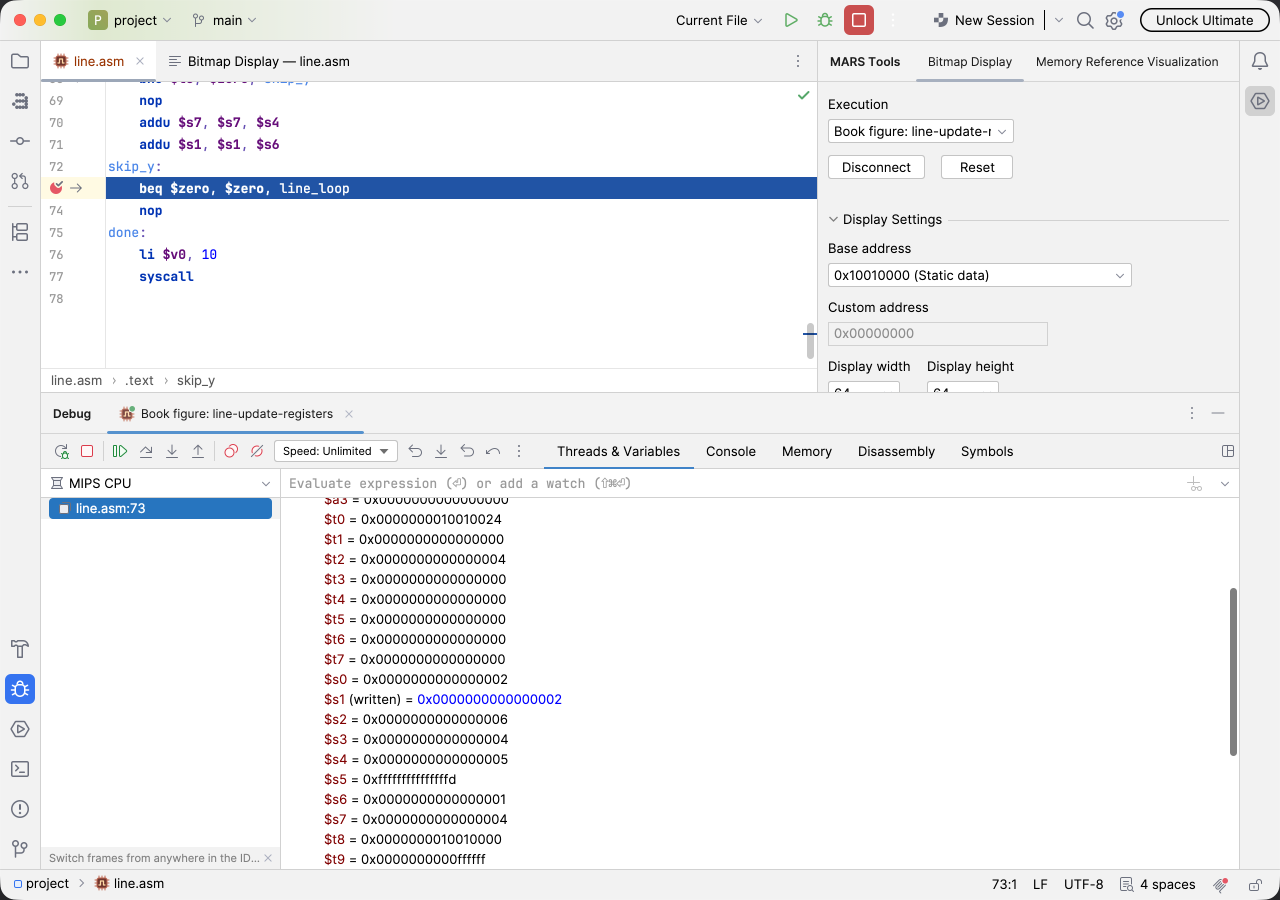
\includegraphics[width=0.4\linewidth,artifact,trim={\MARSupdatestateLeft{} \MARSupdatestateBottom{} \MARSupdatestateRight{} \MARSupdatestateTop{}},clip]{packages/007-bresenham-line/captures/f02-update/registers.png}};
\begin{scope}[shift={(state.south west)},x={($(state.south east)-(state.south west)$)},y={($(state.north west)-(state.south west)$)}]
\draw[black,line width=0.7pt] (0.023529412,0.018072289) rectangle (0.976470588,0.981927711);
\node[draw=black,fill=white,circle,inner sep=1.5pt,font=\footnotesize] at ($(0.023529412,0.981927711)+(-3mm,0)$) {2};
\end{scope}
\node[anchor=north west,inner sep=0,font=\small\bfseries] (plot-title) at ([xshift=0.49\linewidth]state-title.north west) {The image still has one white cell};
\node[anchor=north west,inner sep=0] (plot) at ([yshift=-1mm]plot-title.south west) {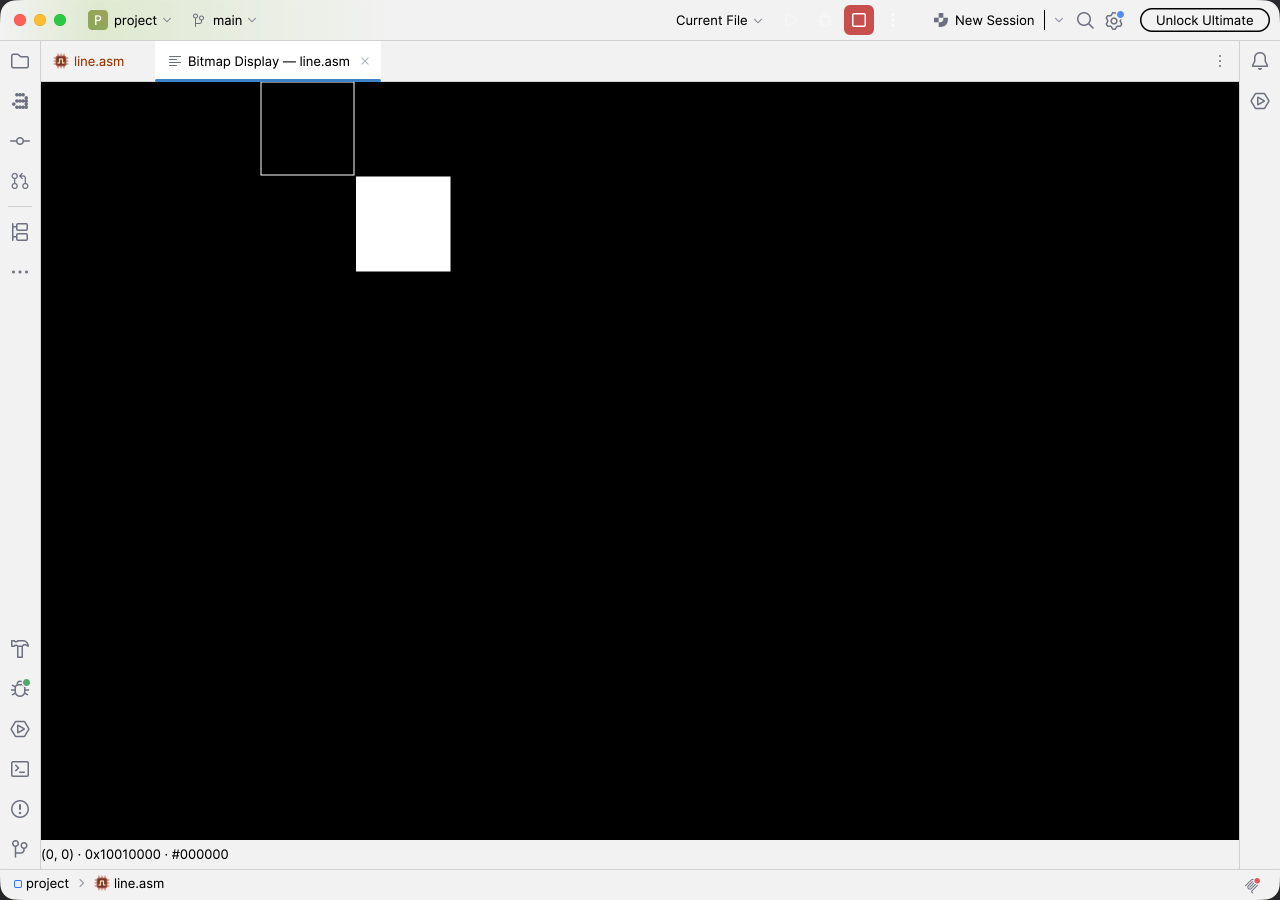
\includegraphics[width=0.32\linewidth,artifact,trim={\MARSupdateplotLeft{} \MARSupdateplotBottom{} \MARSupdateplotRight{} \MARSupdateplotTop{}},clip]{packages/007-bresenham-line/captures/f02-update/bitmap.png}};
\begin{scope}[shift={(plot.south west)},x={($(plot.south east)-(plot.south west)$)},y={($(plot.north west)-(plot.south west)$)}]
\draw[black,line width=0.7pt] (0.000000000,0.000000000) rectangle (1.000000000,1.000000000);
\node[draw=black,fill=white,circle,inner sep=1.5pt,font=\footnotesize] at ($(0.000000000,1.000000000)+(-3mm,0)$) {3};
\foreach \c in {0,...,7} {\node[anchor=north,font=\scriptsize,inner sep=0] at ({(\c+0.5)/8},-0.035) {\c}; \node[anchor=east,font=\scriptsize,inner sep=0] at (-0.025,{1-(\c+0.5)/8}) {\c};}
\node[anchor=north,font=\scriptsize,inner sep=0] at (0.5,-0.11) {$x$}; \node[anchor=east,font=\scriptsize,inner sep=0] at (-0.10,0.5) {$y$};
\end{scope}
\node[anchor=north west,inner sep=0,font=\small\bfseries] (saved-title) at ([yshift=-2mm]state.south west) {Both decisions used the same saved value};
\node[anchor=north west,inner sep=0] (saved) at ([yshift=-1mm]saved-title.south west) {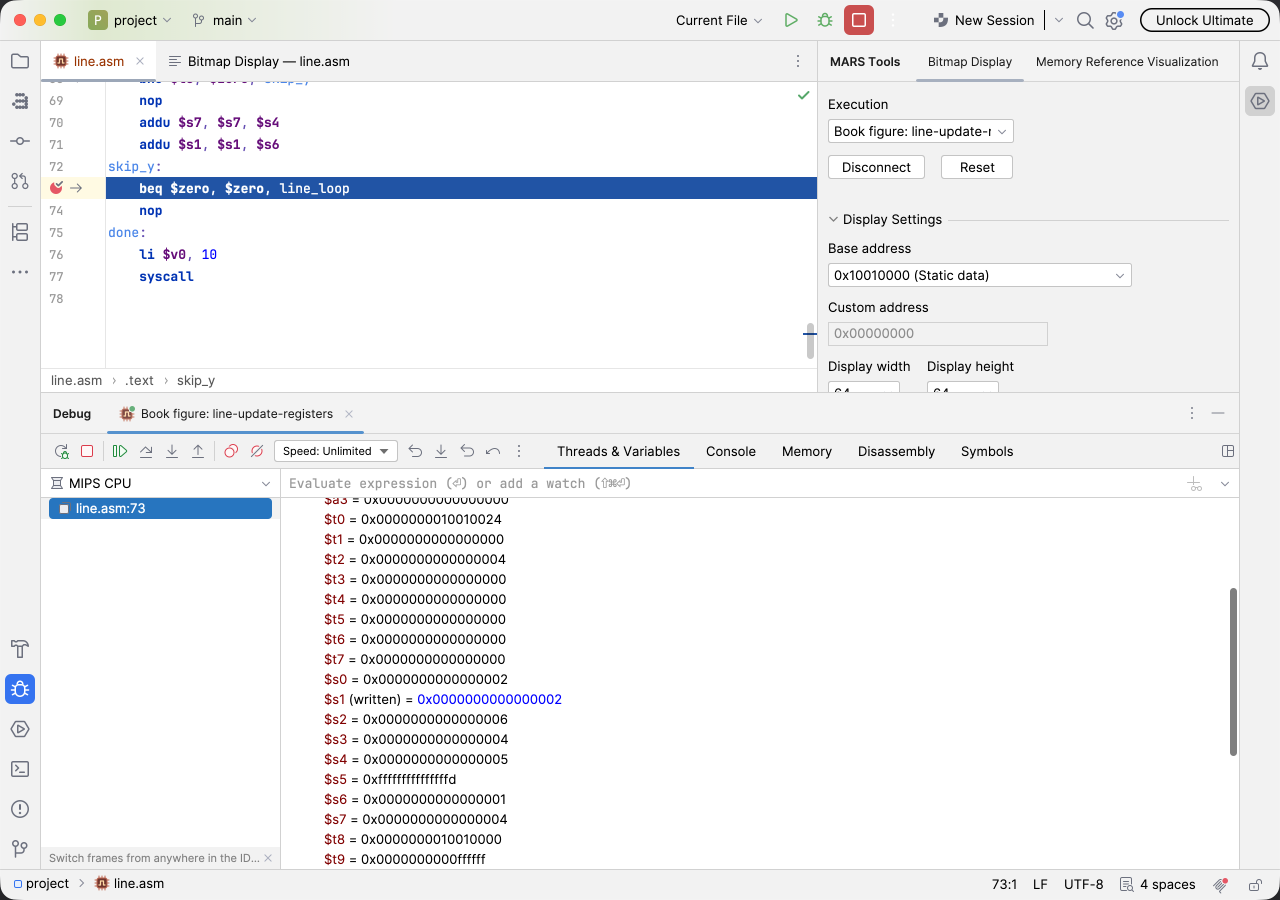
\includegraphics[width=0.4\linewidth,artifact,trim={\MARSupdatesavedLeft{} \MARSupdatesavedBottom{} \MARSupdatesavedRight{} \MARSupdatesavedTop{}},clip]{packages/007-bresenham-line/captures/f02-update/registers.png}};
\begin{scope}[shift={(saved.south west)},x={($(saved.south east)-(saved.south west)$)},y={($(saved.north west)-(saved.south west)$)}]
\draw[black,line width=0.7pt] (0.030150754,0.115384615) rectangle (0.969849246,0.884615385);
\node[draw=black,fill=white,circle,inner sep=1.5pt,font=\footnotesize] at ($(0.030150754,0.884615385)+(-3mm,0)$) {4};
\end{scope}
\end{tikzpicture}
\par\smallskip
\begin{minipage}{\linewidth}
\small
\begin{enumerate}
\item The blue branch returns to \texttt{line\_loop}. Both coordinate updates have completed, but the next address calculation and pixel store lie ahead.
\item The prepared coordinate is $(2,2)$, and the running error is now 4. Starting from 2, the x update adds $dy=-3$, giving $-1$; the y update then adds $dx=5$, giving 4.
\item The original framebuffer still shows only $(1,1)$. Changing the working registers does not paint the next cell. This bitmap is intentionally identical to the previous one even though the instruction boundary and register state differ.
\item \texttt{\$t2}=4 is the saved $e_2=2\cdot2$ from before either update. It satisfied $4\geq-3$ and $4\leq5$, so both coordinates advanced. Its equality with the \emph{new} error 4 is a coincidence; recomputing twice the new error would give 8.
\end{enumerate}
\end{minipage}
\caption{The first update prepares coordinate (2,2). The next loop iteration has not painted that cell yet.}
\label{capture:007-bresenham-line-f02-update}
\end{figure}
\par
